\documentclass[11pt]{article}
\usepackage[margin=1in]{geometry}
\usepackage{amsmath,amssymb,graphicx,booktabs,bm,amsthm,enumitem,cite}
\usepackage[hidelinks]{hyperref}

% Evidence-gated primary-paper macros.
% Evidence-gated result placeholders for the primary manuscript.
% These macros are intentionally non-numeric until the Stage 15 decision gate
% records a reviewed PROCEED or PIVOT.  Replace them only through the evidence-freeze workflow
% documented in docs/research_protocol.md.
\newcommand{\PendingStageFifteen}{\textsc{Pending--Stage 15}}
\newcommand{\ResultHeadline}{\PendingStageFifteen}
\newcommand{\ResultPrimaryAssociation}{\PendingStageFifteen}
\newcommand{\ResultIncrementalValue}{\PendingStageFifteen}
\newcommand{\ResultRankWeightStability}{\PendingStageFifteen}
\newcommand{\ResultExternalAssociation}{\PendingStageFifteen}
\newcommand{\ResultModelCoverage}{\PendingStageFifteen}
\newcommand{\ResultBootstrapUncertainty}{\PendingStageFifteen}
\newcommand{\ResultConclusion}{\PendingStageFifteen}

% Historical macros are loaded only for the quarantined legacy supplement.
% They must never be cited as evidence for the refactored primary claim.
% AUTO-GENERATED by paper/emit_baseline_table.py -- do not hand-edit numbers.
\newcommand{\PhysMaxAngLo}{43}
\newcommand{\PhysMaxAngHi}{55}
\newcommand{\PhysMinAngLo}{2}
\newcommand{\PhysMinAngHi}{6}
\newcommand{\PhysMidAngLo}{10}
\newcommand{\PhysMidAngHi}{15}
\newcommand{\NTestFair}{800}
\newcommand{\FairSpanPriorQRS}{0.481}
\newcommand{\FairSpanDipQRS}{0.183}
\newcommand{\FairSpanRidgeQRS}{0.167}
\newcommand{\FairSpanUnetQRS}{0.164}
\newcommand{\FairLimbPriorQRS}{0.481}
\newcommand{\FairLimbRidgeQRS}{0.344}
\newcommand{\FairLimbUnetQRS}{0.238}
\newcommand{\FairUnetLimbSpanRatio}{1.46}
\newcommand{\RidgeUnetSpanCI}{$[-0.007,+0.000]$\,mV}
\newcommand{\SpanLimbUnetCI}{$[+0.070,+0.079]$\,mV}
\newcommand{\LadderQual}{a ladder in point estimates (the ridge$\to$U-Net step is within its paired CI)}
\newcommand{\EtaSTVone}{0.330}
\newcommand{\EtaNormVone}{0.740}
\newcommand{\AmbVone}{0.093}
\newcommand{\EtaSTVtwo}{0.712}
\newcommand{\EtaNormVtwo}{0.960}
\newcommand{\AmbVtwo}{0.200}
\newcommand{\EtaSTVthree}{0.553}
\newcommand{\EtaNormVthree}{0.955}
\newcommand{\AmbVthree}{0.155}
\newcommand{\EtaSTVfour}{0.268}
\newcommand{\EtaNormVfour}{0.534}
\newcommand{\AmbVfour}{0.075}
\newcommand{\EtaSTVfive}{0.084}
\newcommand{\EtaNormVfive}{0.170}
\newcommand{\AmbVfive}{0.024}
\newcommand{\EtaSTVsix}{0.027}
\newcommand{\EtaNormVsix}{0.057}
\newcommand{\AmbVsix}{0.007}
\newcommand{\SafetyN}{1498}
\newcommand{\SafetyFallbackPct}{14}
\newcommand{\FpDipolar}{5.3}
\newcommand{\FnDipolar}{45.7}
\newcommand{\TotDipolar}{51.1}
\newcommand{\ErrDipolar}{0.077}
\newcommand{\FpRidge}{1.7}
\newcommand{\FnRidge}{52.1}
\newcommand{\TotRidge}{53.7}
\newcommand{\ErrRidge}{0.076}
\newcommand{\FpOls}{1.7}
\newcommand{\FnOls}{51.8}
\newcommand{\TotOls}{53.5}
\newcommand{\ErrOls}{0.076}
\newcommand{\TotWrongLo}{51.1}
\newcommand{\TotWrongHi}{53.7}
\newcommand{\LWspearQRS}{1.00}
\newcommand{\LWspearQRSlo}{0.88}
\newcommand{\LWantlatQRS}{0.98}
\newcommand{\LWspearST}{0.89}
\newcommand{\LWspearSTlo}{-0.54}
\newcommand{\LWantlatST}{0.77}
\newcommand{\LWspearT}{0.94}
\newcommand{\LWspearTlo}{-0.66}
\newcommand{\LWantlatT}{0.72}
\newcommand{\LWSTTstable}{no}
\newcommand{\CalCov}{0.91}
\newcommand{\CalCovLo}{0.89}
\newcommand{\CalCovHi}{0.93}
\newcommand{\CalWidth}{0.150}
\newcommand{\WorstSubCov}{0.72}
\newcommand{\WorstSubName}{HYP}
\newcommand{\WorstSubN}{85}

% AUTO-GENERATED by paper/emit_long_results.py -- do not hand-edit numbers.
\newcommand{\CrossNchap}{350}
\newcommand{\CrossNnormal}{81}
\newcommand{\CrossMNQRSang}{14}
\newcommand{\CrossMNQRSCI}{[10,25]}
\newcommand{\CrossMNSTang}{86}
\newcommand{\CrossMNSTCI}{[57,90]}
\newcommand{\CrossMNTang}{81}
\newcommand{\CrossMNTCI}{[54,89]}
\newcommand{\CrossMNLimbRankPtb}{2}
\newcommand{\CrossMNLimbRankChap}{2}
\newcommand{\CrossMNKapSpanPtb}{2.4}
\newcommand{\CrossMNKapSpanChap}{2.3}
\newcommand{\CrossARQRSang}{14}
\newcommand{\CrossARQRSCI}{[9,31]}
\newcommand{\CrossARSTang}{81}
\newcommand{\CrossARSTCI}{[31,90]}
\newcommand{\CrossARTang}{70}
\newcommand{\CrossARTCI}{[39,89]}
\newcommand{\CrossARLimbRankPtb}{2}
\newcommand{\CrossARLimbRankChap}{2}
\newcommand{\CrossARKapSpanPtb}{2.3}
\newcommand{\CrossARKapSpanChap}{2.3}
\newcommand{\CrossVerdict}{cohort-specific}
\newcommand{\NegDrhoone}{-0.026}
\newcommand{\NegStdone}{0.016}
\newcommand{\NegDrhotwo}{-0.006}
\newcommand{\NegStdtwo}{0.027}
\newcommand{\NegDrhofour}{+0.041}
\newcommand{\NegStdfour}{0.037}
\newcommand{\NegDrhosix}{+0.072}
\newcommand{\NegStdsix}{0.044}
\newcommand{\NegSeeds}{5}
\newcommand{\NegNtest}{800}
\newcommand{\NegCIlo}{+0.011}
\newcommand{\NegCIhi}{+0.134}
\newcommand{\NegCIcovers}{no}
\newcommand{\RealPSDVtwoLo}{1.88}
\newcommand{\RealPSDVtwoHi}{2.25}
\newcommand{\RealAmpVtwoLo}{0.45}
\newcommand{\RealAmpVtwoHi}{0.83}
\newcommand{\OracleRhoVtwoLo}{0.49}
\newcommand{\OracleRhoVtwoHi}{0.55}
\newcommand{\OracleRhoLatLo}{0.21}
\newcommand{\OracleRhoLatHi}{0.34}


\newcommand{\LegacyBanner}{%
  \begin{center}
  \fbox{\parbox{0.92\linewidth}{\textbf{Legacy supplement---not evidence for the primary
  claim.} This material records an earlier research branch.  It is excluded from the
  Stage~15 claim--evidence decision and from the four-page submission.}}
  \end{center}}

\title{\textbf{Robust Target-Specific Recoverability Maps for Reduced-Lead ECG
Reconstruction}\\[2pt]\large Evidence-gated extended protocol and legacy research record}
\newif\ifanon\anontrue
\ifanon
  \author{Anonymous authors\\Paper under double-blind review}
\else
  \author{Weiping Yan\\University of Minnesota, Twin Cities}
\fi
\date{}

\begin{document}
\maketitle

\begin{abstract}
Reduced-lead electrocardiogram (ECG) reconstruction is commonly assessed only after a model
produces a waveform.  We propose a training-set diagnostic that maps each observed configuration,
waveform segment, and target lead to a continuous recoverability score.  The score combines target
geometry outside the observed-row span with within-span amplification, then aggregates over a
prespecified family of rank, lead-weighting, and patient-bootstrap fits.  The sole primary empirical
claim is that this robust map predicts held-out target-lead reconstruction error beyond simple
configuration and signal-scale covariates, across reconstruction families and on an external
cohort.  Numerical claims are withheld pending the Stage~15 evidence decision.  This extended
document separates the new protocol from earlier conditional theory, calibration, clinical-event,
lead-selection, and diffusion branches, which are retained only as a transparent legacy supplement.
\end{abstract}

\section{Research question and contribution}
Reduced-lead acquisition motivates fixed transforms, regression, and learned completion models
\cite{edenbrandt1988dower,kors1990vcg,nelwan2004reduced,gradowski2025reveals,%
cardoso2024bayesian,lence2025ecgrecover,fang2026imputeecg,pagotto2025minimal}.  These methods answer
how to synthesize a missing waveform.  We ask a complementary question: before selecting a
reconstructor, can training-set spatial geometry anticipate which segment and target lead will have
larger held-out error?

The refactored paper has one claim and one falsification route.  For each observed set $S$, segment
$s$, and target lead $\ell$, a frozen robust score should (i) rank held-out target error, (ii) add
out-of-sample predictive value beyond lead count, configuration rank, target scale, pairwise
correlation, and global conditioning, (iii) retain its direction across transparent and learned
reconstructors, and (iv) retain its direction on a second cohort.  Failure of the incremental,
cross-model, or external tests prevents a positive headline.  The score is described as a map or
diagnostic; it is not a clinical guarantee or a claim about all information in an ECG waveform.

\section{Robust target-specific map}
\label{sec:primary-method}
Let $\bm x_{i,s}(t)\in\mathbb R^p$ be the multilead signal for patient $i$ in segment $s$.  A
training-only weighted covariance fit gives $\bm M_s^v\in\mathbb R^{p\times r}$, with
$v=(r,w,b)$ indexing candidate rank, lead weighting, and patient-bootstrap replicate.  For target
row $\bm m_{s,\ell}^v$ and observed rows $\bm M_{s,S}^v$, define
\begin{align}
u_{s,\ell}^{v}(S)&=
\frac{\|\bm m_{s,\ell}^{v}[\bm I-(\bm M_{s,S}^{v})^+\bm M_{s,S}^{v}]\|_2}
{\|\bm m_{s,\ell}^{v}\|_2+\epsilon},\\
g_{s,\ell}^{v}(S)&=\|\bm m_{s,\ell}^{v}(\bm M_{s,S}^{v})^+\|_2,\\
q_{s,\ell}^{v}(S)&=
\left[(u_{s,\ell}^{v})^2+
\left\{\frac{\nu_{s,S}^{v}g_{s,\ell}^{v}}
{\sigma_{s,\ell}^{v}+\epsilon}\right\}^{2}\right]^{1/2},
\label{eq:robust-score-long}
\end{align}
where $\nu$ is a training-only observed residual scale and $\sigma$ a training-only target scale.
The first term measures target geometry absent from the observed-row span of the fitted
representation; the second measures amplification relative to target scale.  The primary map is the
median $q^v$ over plausible fits, accompanied by patient-bootstrap quantiles.  Its empirical value
comes only from the held-out tests below.

\paragraph{Prespecified perturbations.}
The primary fit uses eight algebraically independent measured channels; the 12 displayed leads form
a weighting sensitivity.  Folds 1--7 fit rank candidates $2$--$5$, fold~8 chooses the primary rank
by an out-of-sample representation criterion, and all plausible ranks remain in the envelope.
Patient-cluster bootstrap resamples refit the subspace.  Sign conventions, units, segment windows,
pseudoinverse tolerance, and missing-segment rules are frozen before fold~10 is opened.

\section{Evaluation and analysis contract}
\label{sec:primary-eval}
\paragraph{Split discipline and cohorts.}
PTB-XL official folds 1--7 are used for fitting, fold~8 for design choices, fold~9 for a full pipeline
rehearsal without claim selection, and fold~10 once for the primary evaluation
\cite{wagner2020ptbxl}.  The Chapman--Shaoxing--Ningbo cohort is the external test and uses the
frozen PTB-XL specification \cite{zheng2020chapman}.  The patient is the resampling unit.  QRS, ST,
and T form the core analysis; P-wave results move to the supplement if the frozen delineation-quality
criterion is not met.

\paragraph{Reconstruction families.}
Prior mean and ridge regression are transparent anchors.  A mask-conditioned 1-D U-Net represents a
flexible learned family.  Stage~15 also requires at least one reproducible public strong-method
adapter; ECGrecover and ImputeECG are prioritized subject to artifact, license, and protocol
compatibility \cite{lence2025ecgrecover,fang2026imputeecg}.  All reconstructors receive the same
observed samples and mask.  Seeds, checkpoints, preprocessing, failures, and unavailable-method
reasons are retained.

\paragraph{Primary endpoint and test.}
The primary outcome is patient-level target-lead normalized RMSE within segment.  For
$(S,s,\ell,\text{reconstructor})$ cells, we first report rank association with the frozen map.  We
then compare a baseline predictive model containing lead count, configuration rank, target RMS,
maximum pairwise correlation, and global conditioning against the same model plus $q$.  Incremental
out-of-sample fit, coefficient direction, and patient-cluster bootstrap intervals are co-primary
evidence.  Segment- and model-specific contrasts are secondary and multiplicity controlled.
External validation tests the frozen score--error relationship; subspace-angle agreement alone is
insufficient.

\begin{table}[t]
\centering
\caption{Primary claim--evidence matrix before the Stage~15 decision.}
\label{tab:primary-evidence-long}
\begin{tabular}{p{0.43\linewidth}p{0.22\linewidth}p{0.24\linewidth}}
\toprule
Evidence item & Gate value & Failure consequence \\
\midrule
Held-out score--error association & \ResultPrimaryAssociation & No positive primary claim \\
Increment beyond simple covariates & \ResultIncrementalValue & Recast as descriptive map \\
Rank/weight/bootstrap stability & \ResultRankWeightStability & Narrow supported scope \\
External-cohort association & \ResultExternalAssociation & No transfer language \\
Coverage across model families & \ResultModelCoverage & Model-specific conclusion \\
Patient-level uncertainty & \ResultBootstrapUncertainty & Evidence gate fails \\
\bottomrule
\end{tabular}
\end{table}

\section{Evidence gates, reproducibility, and decision policy}
Stage~5 requires a verified literature ledger and a novelty statement that distinguishes the map
from reconstruction methods.  Stage~9 freezes splits, endpoints, covariates, reconstructors,
perturbations, exclusions, seeds, and decision rules.  Stage~15 permits \textsc{Proceed} only after
a real non-simulated run provides immutable run identifiers, clean source state, dataset and split
hashes, checkpoint hashes, leakage tests, patient-cluster uncertainty, a strong public baseline,
external validation, and a completed claim--evidence matrix.  Stage~20 additionally requires no
pending macros, verified citations, readable figures, a clean manuscript build, and a strict release
audit.  \textsc{Refine} and \textsc{Pivot} are valid outcomes; negative and failed runs remain in the
record.  The detailed contract is maintained in \texttt{docs/research\_protocol.md}.

\section{Limitations and current status}
The map is built from a fitted linear representation, while flexible models may exploit nonlinear
population regularities.  Delineation, pathology mix, devices, noise, and lead placement can change
both geometry and error.  One external cohort is not deployment validation, and waveform similarity
is not diagnostic or clinical equivalence.  The current empirical status is deliberately
\ResultPrimaryAssociation: the protocol is ready for gated execution, but it does not yet support a
numerical abstract or a positive performance conclusion.

\section{Conclusion}
The intended contribution is a narrow, falsifiable diagnostic: a robust target-specific map that
predicts held-out reconstruction difficulty beyond simple baselines and complements direct model
benchmarking.  Its headline is conditional on the Stage~15 evidence decision.  The following pages
retain earlier branches for auditability, separated from the primary narrative and evidence chain.

\clearpage
\appendix
\section{Legacy supplement: conditional fixed-rank analysis}
\label{app:legacy-theory}
\LegacyBanner
The material in this section assumes a fixed low-rank representation and studies conditional
algebraic properties.  It is retained to preserve research history, not to justify the robust
map--error hypothesis in the main paper.
% Exact per-target-lead identifiability (exact pseudo-inverse) vs the deployed rho-truncated
% numerical map. No residual-independence claim on real data; the strict lower bound is stated
% only for the synthetic model (Proposition 2).

\newtheorem{theoremc}{Proposition}
\newtheorem{propc}[theoremc]{Proposition}

% ---------------------------------------------------------------- setup
\noindent\textbf{Model.} Within segment $s$ write the population 12-lead vector as
$\bm L_s = \bm\mu_s + \bm M_s\bm d + \bm r_s$, where $\bm M_s\in\mathbb R^{12\times3}$
is the (population-estimated, PCA) dipolar basis, $\bm d$ the dipole coordinates, and
$\bm r_s$ the non-dipolar residual. Observing $S$ gives $\bm y_S=\bm{\mathrm{Sel}}_S\bm L_s
+\bm n$, with $\bm M_{s,S}=\bm{\mathrm{Sel}}_S\bm M_s$. Write the exact Moore--Penrose
pseudo-inverse $\bm M_{s,S}^{+}$ and the exact row-space projector
$\bm P_{\mathrm{obs}}=\bm M_{s,S}^{+}\bm M_{s,S}$. For numerical deployment we also use the
\emph{rank-$r$ truncation} at relative tolerance $\varrho$,
$\bm M_{s,S}^{(\varrho)}=\bm U_r\bm\Sigma_r\bm V_r^{\top}$ keeping singular triplets with
$\sigma_i>\varrho\,\sigma_{\max}$, with pseudo-inverse $\bm M_{s,S}^{(\varrho)+}$ and projector
$\bm P_{\mathrm{obs}}^{(\varrho)}=\bm V_r\bm V_r^{\top}$.

% ---------------------------------------------------------------- exact theorem
\begin{theoremc}[Exact per-target-lead dipolar identifiability and conditioning]
\label{thm:perlead}
For each target lead $\ell$ define
$\eta_{s,\ell}(S)=\big\|\bm e_\ell^{\top}\bm M_s(\bm I-\bm P_{\mathrm{obs}})\big\|_2$ and
$\kappa_{s,\ell}(S)=\big\|\bm e_\ell^{\top}\bm M_s\bm M_{s,S}^{+}\big\|_2$ from the \emph{exact}
$\bm M_{s,S}$.
\begin{enumerate}
\item[(i)] \emph{Identifiability.} $\eta_{s,\ell}(S)=0$ iff $\bm e_\ell^{\top}\bm M_s$ lies in
the exact row space of $\bm M_{s,S}$; then $\bm e_\ell^{\top}\bm M_s\bm d$ is a deterministic
function of $\bm M_{s,S}\bm d$---two dipoles with the same observation have the same lead-$\ell$
dipolar value, at any SNR. If $\eta_{s,\ell}(S)>0$ there is a $\bm\delta\in\ker\bm M_{s,S}$
(an unobserved dipole direction) with $\bm e_\ell^{\top}\bm M_s\bm\delta\neq0$; then $\bm d$ and
$\bm d+t\bm\delta$ produce identical observations for all $t$ while lead $\ell$'s dipolar value
changes, so it is not identifiable at any SNR.
\item[(ii)] \emph{Conditioning.} On the identifiable part, the lead-$\ell$ error from
observation noise and observed non-dipolar residual obeys
$\big|\bm e_\ell^{\top}\bm M_s\bm M_{s,S}^{+}(\bm{\mathrm{Sel}}_S\bm r_s+\bm n)\big|
\le \kappa_{s,\ell}(S)\,\big(\|\bm{\mathrm{Sel}}_S\bm r_s\|_2+\|\bm n\|_2\big).$
\end{enumerate}
The global $\kappa_s(S)=\|\bm M_s\bm M_{s,S}^{+}\|_2$ (spectral norm) upper-bounds every per-lead
$\kappa_{s,\ell}(S)$ (a row norm never exceeds the spectral norm; it is not their maximum).
\end{theoremc}

\noindent\emph{Exact vs.\ $\varrho$-identifiability (numerical deployment).} The deployed map
computes $\eta^{(\varrho)}_{s,\ell},\kappa^{(\varrho)}_{s,\ell}$ from the truncation
$\bm P_{\mathrm{obs}}^{(\varrho)}$, so a singular direction observed only through a value below
$\varrho\,\sigma_{\max}$ is treated as unobserved. Then $\eta^{(\varrho)}_{s,\ell}>0$ means lead
$\ell$ is \emph{not stably recoverable at resolution $\varrho$} (outside the retained numerical
row space); it does \emph{not} by itself imply the exact matrix has a null direction---a
tiny-but-nonzero singular value is exactly identifiable ($\eta=0$) yet $\varrho$-unidentifiable
($\eta^{(\varrho)}>0$), as we verify numerically (\texttt{tests/test\_exact\_vs\_rho.py}). We therefore call the
$\eta^{(\varrho)}$ heatmap the \emph{$\varrho$-identifiability} map; for well-separated
configurations the exact and $\varrho$ verdicts coincide, and near-rank-deficient $S$ are
reported with a $\varrho$-sweep and record-bootstrap CIs. \textbf{The limb-6 flagship is exact:}
the six limb leads are exact linear combinations of I and II (Einthoven/Goldberger), so
$\bm M_{s,S}$ has exact rank~2 and precordial ST is \emph{exactly} non-identifiable from limb
leads at any SNR, independent of $\varrho$.

\noindent\emph{Relation to classical estimability.} Part~(i) is the classical estimability
criterion (Gauss--Markov / \cite{scheffe1959anova}) for the linear functional
$\bm e_\ell^{\top}\bm M_s\bm d$; we claim no novelty for this identity. The contribution
(Sec.~\ref{sec:exp}) is its use as a graded, empirically-estimated recoverability map with
per-record calibrated error rates (Sec.~\ref{sec:calib}).

% ---------------------------------------------------------------- residual (honest)
\noindent\textbf{The non-dipolar residual (no independence claim on real data).}
Let $\bm m_s(\bm y_S)=\mathbb E[\bm r_s\mid\bm y_S]$ and
$\bm u_s=\bm r_s-\bm m_s(\bm y_S)$, so $\mathbb E[\bm u_s\mid\bm y_S]=\bm 0$. We do
\emph{not} assume $\bm u_s\perp\bm y_S$. Under squared loss the Bayes-optimal reconstruction
error of the (vector) residual is
\[
\inf_{\hat{\bm r}}\ \mathbb E\big\|\bm r_s-\hat{\bm r}(\bm y_S)\big\|_2^2
=\mathbb E\big[\operatorname{tr}\operatorname{Cov}(\bm r_s\mid\bm y_S)\big].
\]
Part of $\bm r_s$ (the \emph{empirically predictable residual}) is recovered by a
predictor trained on $\bm y_S$ and metered with distribution-free calibrated intervals;
the remainder is an \emph{achievability gap}, established by a held-out achievability
analysis for a stated predictor family---\emph{not} declared unrecoverable a priori.

\begin{propc}[Strict independence limit -- synthetic model only]
\label{prop:synth}
If the data are generated so that a component $\bm u$ is statistically independent of
$\bm y_S$ (an explicit synthetic construction), then $p(\bm u\mid\bm y_S)=p(\bm u)$, the
Bayes estimate of $\bm u$ under squared loss is its prior mean, and
$\mathbb E\|\widehat{\bm u}-\bm u\|_2^2\ge\operatorname{tr}\operatorname{Cov}(\bm u)$ for any
estimator. This strict limit is invoked \emph{only} for the synthetic model; on real ECG we
make no such independence claim.
\end{propc}

\subsection*{A certified minimax recoverability floor}
\label{sec:floor}
Proposition~\ref{thm:perlead} says \emph{whether} a target lead's dipolar coordinate is recoverable
($\eta{=}0$) and \emph{how well-conditioned} the estimate is ($\kappa$). We now turn the binary
verdict into a \emph{quantitative} per-lead risk floor in physical units that lower-bounds
\emph{every} reconstructor, linear or learned. Fix segment $s$ and observed set $S$; write the
dipole prior second moment $\bm\Sigma_d=\mathbb E[\bm d\bm d^\top]$, the observed-dipole row-space
projector $\bm P=\bm M_{s,S}^{+}\bm M_{s,S}$, and $\bm Q=\bm I-\bm P$. The target is the dipolar
functional of lead $\ell$, $\theta_\ell=\bm e_\ell^\top\bm M_s\bm d$, and the prior-conditional
ambiguity of Sec.~\ref{sec:cert} is
\[
a_{s,\ell}(S)^2 \;=\; \bm e_\ell^\top\bm M_s\,\bm\Sigma_{Q\mid P}\,\bm M_s^\top\bm e_\ell,
\qquad
\bm\Sigma_{Q\mid P}=\bm Q\bm\Sigma_d\bm Q-\bm Q\bm\Sigma_d\bm P(\bm P\bm\Sigma_d\bm P)^{+}\bm P\bm\Sigma_d\bm Q .
\]

\begin{theoremc}[Minimax per-lead recoverability floor]\label{thm:floor}
Let $\mathcal P(\bm\Sigma_d)=\{\pi:\ \mathbb E_\pi[\bm d\bm d^\top]\preceq\bm\Sigma_d\}$ be the class of
priors with second moment dominated by $\bm\Sigma_d$.
\begin{enumerate}[label=(\roman*),leftmargin=1.6em]
\item \textbf{Noise-free dipolar floor (nonlinear estimators).} For \emph{any} estimator
$\hat\theta_\ell(\bm y_S)$ (measurable, possibly nonlinear/learned) of $\theta_\ell$ from the exact
observation $\bm y_S=\bm M_{s,S}\bm d$,
\[
\inf_{\hat\theta_\ell}\ \sup_{\pi\in\mathcal P(\bm\Sigma_d)}\ \mathbb E_\pi\big[(\hat\theta_\ell-\theta_\ell)^2\big]
\;=\; a_{s,\ell}(S)^2 ,
\]
attained by the least-favourable Gaussian prior $\mathcal N(\bm 0,\bm\Sigma_d)$ and its linear
posterior-mean estimator. In particular $a_{s,\ell}(S)^2=0$ iff $\eta_{s,\ell}(S)=0$, and every
reconstructor incurs risk $\ge a_{s,\ell}(S)^2$ under the least-favourable prior in the class.
\item \textbf{Noise/residual inflation.} With observed noise and non-dipolar residual of covariance
$\bm N$ on $S$, the risk floor lifts to
$a_{s,\ell}(S)^2+\lambda_{\min}$-scale term bounded through
$\kappa_{s,\ell}(S)=\|\bm e_\ell^\top\bm M_s\bm M_{s,S}^{+}\|_2$: the amplified error is
$\bm e_\ell^\top\bm M_s\bm M_{s,S}^{+}(\bm{\mathrm{Sel}}_S\bm r_s+\bm n)$, of variance
$\le\kappa_{s,\ell}(S)^2\,\|\bm N\|_2$ (Prop.~\ref{thm:perlead}(ii)).
\item \textbf{Finite-sample subspace floor.} With $\bm M_s$ replaced by its rank-3 PCA estimate
$\widehat{\bm M}_s$ from $N$ records,
$\big|a_{s,\ell}(S;\widehat{\bm M}_s)^2-a_{s,\ell}(S;\bm M_s)^2\big|\le C\,\sin\Theta(\widehat{\bm M}_s,\bm M_s)\,\|\bm\Sigma_d\|_2$,
where $\sin\Theta$ is the principal-angle perturbation (Davis--Kahan~\cite{davis1970rotation}). The
conservative floor $a^{-}_{s,\ell}(S)=\min$ over the record-bootstrap confidence set of
$\widehat{\bm M}_s$ then lower-bounds the risk uniformly in the estimated subspace.
\end{enumerate}
\end{theoremc}

\noindent\emph{Proof sketch.} (i) Gaussian conditioning gives
$\mathrm{Var}(\theta_\ell\mid\bm P\bm d)=\bm e_\ell^\top\bm M_s\bm\Sigma_{Q\mid P}\bm M_s^\top\bm e_\ell$
with the posterior mean Bayes-optimal under squared loss, so the Bayes risk equals $a_{s,\ell}^2$;
estimating the \emph{linear} functional $\theta_\ell=\bm e_\ell^\top\bm M_s\bm d$ under a
convex, quadratically-constrained parameter class makes the nonlinear minimax risk equal the linear
one, with a least-favourable Gaussian prior (Donoho--Liu~\cite{donohoLiu1991}; Donoho, optimal
recovery~\cite{donoho1994}), giving the sup--inf identity and the bound for arbitrary $\hat\theta_\ell$.
(ii) Cauchy--Schwarz/$\sigma_{\min}$ on the amplified-error term, as in
Prop.~\ref{thm:perlead}(ii). (iii) Weyl/Davis--Kahan perturbation of the projectors and Schur
complement as functions of $\widehat{\bm M}_s$, propagated through the quadratic form.\hfill$\square$

\smallskip
\noindent\textbf{What is and is not certified.} The floor is \emph{minimax over the moment class}
$\mathcal P(\bm\Sigma_d)$, not distribution-free: a reconstructor exploiting higher moments the true
(non-Gaussian) $\bm d$ happens to carry could beat $a_{s,\ell}^2$ under the \emph{true} prior, not
the least-favourable one. The certified quantity is the \emph{dipolar} functional $\theta_\ell$,
where the algebra is exact; a floor on the \emph{full} lead $\bm e_\ell^\top\bm L_s$ would require
bounding $\operatorname{tr}\mathrm{Cov}(\bm r_\ell\mid\bm y_S)$, which we decline to certify and
instead meter empirically with the distribution-free intervals of Sec.~\ref{sec:calib}. So
``no estimator beats $a_{s,\ell}(S)$ over the moment class'' is a target-specific, finite-sample
statement about the identifiable dipolar component; we verify it numerically under the
least-favourable Gaussian prior (\texttt{tests/test\_floor.py}: zero floor violations). On real ECG
the floor is \emph{operational and tight}: the theoretical ambiguity $a_{s,\ell}$ strongly predicts
the measured per-lead dipolar error (Spearman $\CertValSpearAmb$, Pearson $\CertValPearAmb$;
Fig.~\ref{fig:certval}), the identifiable/unidentifiable split is separated with AUC
$\CertValAUC$, and the pure-dipolar reconstructor is bounded by the floor while data-driven
reconstructors sit right at it (median gap $\CertValFloorGap$\,mV)---beating the moment-class worst
case only marginally by exploiting non-Gaussian population structure, exactly the residual the
calibrated intervals of Sec.~\ref{sec:calib} meter. This turns the empirically similar total error
across reconstructors (Sec.~\ref{sec:exp}) into a target-specific certified minimax floor.
Crucially the floor also binds a \emph{learned} reconstructor: a trained arbitrary-mask diffusion
model (DDPM, honest guidance $w{=}1$), evaluated against the \emph{same} floor on held-out records,
sits above it in every one of $\FloorDiffNcells$ underdetermined cells (floor-violation fraction
$\FloorDiffViol$, median gap $\FloorDiffGap$\,mV), and the certificate's identifiable/unidentifiable
split predicts its error---median dipolar-projection RMSE $\FloorDiffEtaZero$\,mV where
$\eta{=}0$ versus $\FloorDiffEtaPos$\,mV where $\eta{>}0$ (\texttt{experiments/certificate\_floor\_diffusion.py}).
Notably the generative model does \emph{not} beat the moment-class floor at all, whereas the linear
ridge does on a minority of cells---the worst-case bound is loose only for the estimator explicitly
exploiting the non-Gaussian structure it excludes.

\subsection*{Cross-cohort transfer of the recoverability verdict}
\label{sec:transfer}
The certificate is computed from a \emph{fitted} dipolar subspace $\bm M_s$ (the rank-3 PCA of one
cohort's segment-$s$ samples). A natural worry is that the verdict is an artefact of the fitting
cohort. It is not: because $\eta_{s,\ell}(S)=\|\bm e_\ell^\top\bm M_s(\bm I-\bm P_{\mathrm{obs}})\|_2$
depends on $\bm M_s$ \emph{only through its column space}, it is invariant to any rotation of the
$3$-dimensional dipole basis, and drifts across cohorts only as fast as the two cohorts' dipolar
\emph{subspaces} separate.

\begin{theoremc}[Cross-cohort transfer bound]\label{thm:transfer}
Let cohorts $A,B$ have segment-$s$ dipolar bases $\bm M_s^A,\bm M_s^B\in\mathbb R^{12\times3}$ with
orthonormal columns, and let $\theta^\star$ be the largest principal angle between
$\operatorname{col}(\bm M_s^A)$ and $\operatorname{col}(\bm M_s^B)$. For every target lead $\ell$
and observed set $S$,
\[
\big|\eta_{s,\ell}^A(S)-\eta_{s,\ell}^B(S)\big|
\;\le\; 2\sin(\theta^\star/2)\,\big(1+2\,\kappa_{s}(S)\big),
\qquad \kappa_s(S)=\|\bm M_{s,S}^{+}\|_2=\|\bm M_s\bm M_{s,S}^{+}\|_2 ,
\]
the observed-set conditioning of Prop.~\ref{thm:perlead}. In particular $\theta^\star{=}0$ gives
$\eta^A_{s,\ell}(S)=\eta^B_{s,\ell}(S)$ exactly.
\end{theoremc}

\noindent\emph{Proof sketch.} $\eta$ is unchanged if $\bm M_s$ is right-multiplied by any
$\bm R\in O(3)$ (it rotates $\bm P_{\mathrm{obs}}$ and $\bm e_\ell^\top\bm M_s$ together), so align the
bases by the optimal $\bm R$, giving $\|\bm M_s^A-\bm M_s^B\|_2=2\sin(\theta^\star/2)=:\delta$. With
$\bm m_\ell=\bm M_s^\top\bm e_\ell$ ($\|\bm m_\ell\|\le1$) and $\bm P_S$ the row-space projector,
$\big|\,\|(\bm I{-}\bm P_S^A)\bm m_\ell^A\|-\|(\bm I{-}\bm P_S^B)\bm m_\ell^B\|\,\big|
\le\|\bm m_\ell^A-\bm m_\ell^B\|+\|\bm P_S^A-\bm P_S^B\|_2\,\|\bm m_\ell^B\|
\le\delta+2\delta\kappa_s(S)$, using the projector perturbation
$\|\Delta\bm P_S\|_2\le2\|\Delta\bm M_{s,S}\|_2\|\bm M_{s,S}^{+}\|_2$ (Stewart--Wedin) and
$\|\bm m_\ell^B\|\le1$.\hfill$\square$

\smallskip
\noindent\textbf{What this buys, and its honest limits.} The bound is a $\sin\Theta$ perturbation
(Davis--Kahan~\cite{davis1970rotation}) that makes a \emph{single} extra cohort load-bearing: the
transferability of the verdict is governed by a \emph{computable} quantity---the principal angle
between the cohorts' dipolar subspaces---so a large angle \emph{flags} non-transfer before any
target-cohort label is seen. The constant $1+2\kappa_s$ is worst-case and the bound is loose in
absolute terms (for a well-conditioned observed set it can exceed the trivial $\eta\le1$); its value
is as a \emph{pre-deployment transfer-risk flag}: a small principal angle certifies a small
verdict drift, a large one refuses to. On PTB-XL$\to$Chapman (matched sinus, limb-6 $\to$ V2) the two
regimes are visible. The QRS dipolar subspace is nearly shared
($\theta^\star{=}\TransferAngleQRS^\circ$) and the measured drift is correspondingly tight
($\TransferDriftQRS$, realized slope $\TransferLipQRS$)---the verdict transfers. The ST subspace is
near-orthogonal ($\theta^\star{=}\TransferAngleST^\circ$, CI up to $89.6^\circ$): the bound turns
vacuous and the drift is genuinely uncertain---the target-cohort $\eta$ bootstrap CI is
$[0.02,0.71]$, spanning most of the admissible range, so the realized slope is only pinned to
$[\TransferSTLipLo,\TransferSTLipHi]$ and we claim
\emph{no} precise ST drift, only that the large angle flags the ST verdict as non-transferable
(\texttt{experiments/transfer\_bound.py}). We therefore do not read a stable cross-segment Lipschitz
constant from these two points; the load-bearing claim is the rigorous bound plus the angle as a
computable transfer-risk diagnostic, corroborated by the tight QRS point. This is the cross-cohort
analogue of the finite-sample $\sin\Theta$ term in Thm.~\ref{thm:floor}(iii): both control how a
fitted subspace perturbs the verdict.


\section{Legacy supplement: calibration branch}
\label{sec:calib}
\LegacyBanner
The earlier conformal-calibration branch addresses a different estimand from the robust score and is
outside the primary claim.
\subsection{Calibrated intervals for the predictable residual}
The prediction target is the \emph{record-level segment-mean} off-dipole residual of the target
lead (one scalar per record: the mean over the segment's samples). We train a gradient-boosted
quantile regressor of it on the observed leads' segment means and apply Mondrian conformalized
quantile regression \cite{romano2019cqr} per $(S,s,\ell)$ group, with strict fold discipline:
basis and model on folds 1--7, the regressor's \texttt{max\_iter} selected by pinball loss on
fold 8, conformal calibration on fold 9, and a single evaluation on fold 10 (nominal
$1{-}\alpha{=}0.90$). This is a sound \emph{application} of established conformal machinery, not
a new predictor; the contribution is attaching it, per feature and lead, to the recoverability
map. Across the pre-registered $(S,s,\ell)$ groups, fold-10 within-group
coverage clusters near nominal ($0.87$--$0.94$; e.g.\ $\{$I,II,V1,V3,V5$\}$ QRS/V2
$\CalCov$, record-bootstrap CI $[\CalCovLo,\CalCovHi]$, mean width $\CalWidth$\,mV).

\textbf{What is and is not guaranteed.} Mondrian CQR gives \emph{within-$(S,s,\ell)$-group
marginal} coverage under exchangeability---\emph{not} coverage conditional on diagnosis, which
is not a conditioning variable. Diagnostic subgroups are therefore not guaranteed and the
smallest ones fall below nominal: the worst is the \WorstSubName{} subgroup at coverage
$\WorstSubCov$ ($n{=}\WorstSubN$), the expected finite-sample behaviour when conditioning on
a variable the calibration does not stratify on. We report worst-subgroup coverage rather than
hide it under the aggregate band, and we make no distribution-free claim beyond exchangeability
with the calibration fold.

\section{Legacy supplement: PTB-XL map, event, and baseline studies}
\label{sec:exp}
\LegacyBanner
These analyses use the earlier fixed-rank formulation.  Their values are historical artifacts and
must not populate the refactored manuscript without a new Stage~9 freeze and Stage~15 decision.

\begin{figure}[t]
  \centering
  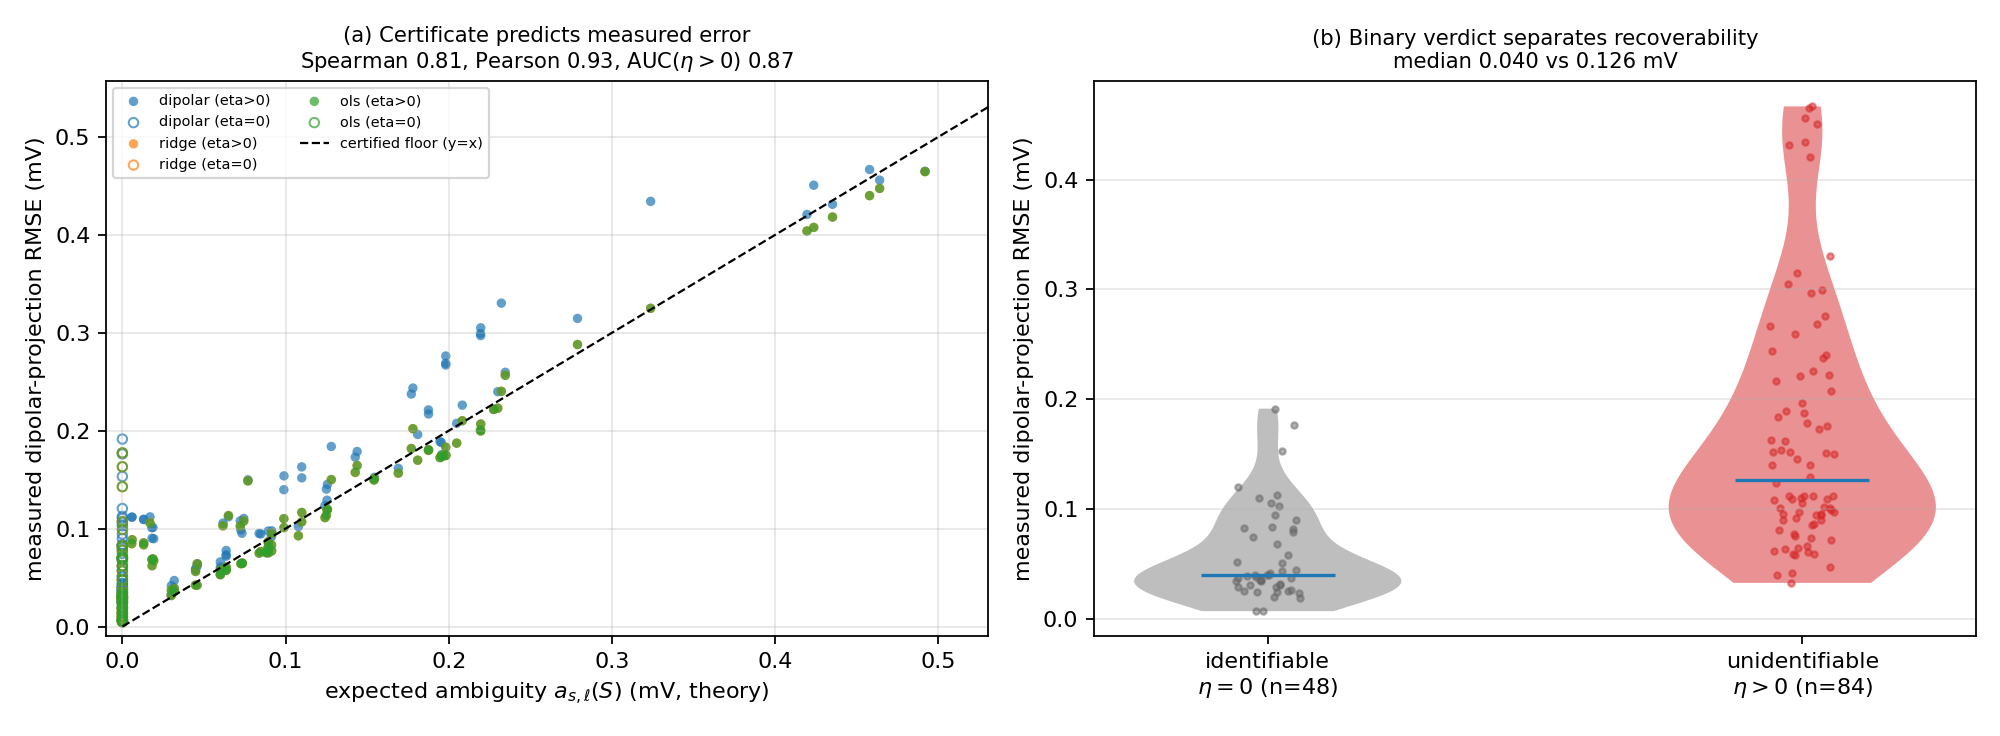
\includegraphics[width=0.92\linewidth]{../results/certificate_validation.png}
  \caption{Legacy diagnostic retained for traceability.  It is not evidence for the robust
  map--error claim and is excluded from the short submission.}
  \label{fig:certval}
\end{figure}
\subsection{The recoverability map on PTB-XL}
We estimate $\bm M_s$ (rank 3; the cardiac dipole is 3-D \emph{a priori}, and the cumulative
explained variance confirms rank~3 captures the bulk---a rank-sensitivity sweep $r{=}2\dots5$ is
reported in \texttt{results/recoverability\_maps.json}) per segment on the training NORM records,
with RECORD-LEVEL bootstrap CIs (resample records, refit $\bm M_s$; $\varrho{=}10^{-2}$;
Fig.~\ref{fig:map}). We plot the \emph{normalized} identifiability
$\tilde\eta_{s,\ell}=\eta_{s,\ell}/\|\bm e_\ell^\top\bm M_s\|_2$---a dimensionless relative
unobserved geometric gain (a ratio of $L_2$ norms, not a variance fraction). A single observed
lead leaves every other lead unidentifiable; a dipole-spanning $\{$I,II,V2$\}$ or
$\{$I,II,V1,V3,V5$\}$ makes all targets \emph{exactly} identifiable ($\eta{=}0$).

\textbf{The robust flagship is exact.} The six limb leads are exact linear combinations of I and
II, so $\bm M_{s,S}$ for limb-6 has \emph{exact} rank 2: precordial ST is \emph{exactly}
non-identifiable from limb leads at any SNR, independent of $\varrho$ (Prop.~\ref{thm:perlead}).

\textbf{Graded ordering: stable for QRS, weighting-sensitive for ST/T.} A duplicated-limb
sensitivity analysis (\texttt{results/lead\_weighting.json}: refit on the 8 algebraically
independent leads, on the \emph{same} records) shows the V1--V6 $\tilde\eta$ ordering is
bootstrap-stable for QRS (Spearman $\LWspearQRS$, CI lower bound $\LWspearQRSlo$;
anterior-before-lateral in $\LWantlatQRS$ of resamples) but \emph{not} robust for the
low-amplitude ST/T segments (ST Spearman point $\LWspearST$ with a wide bootstrap CI;
anterior-before-lateral in only $\LWantlatST$ of resamples). We therefore report the ST/T
$\tilde\eta$/ambiguity magnitudes with this caveat and \emph{do not} claim a fine ST/T ordering;
the binary limb$\to$precordial verdict above is the robust ST statement. The estimated subspace
also depends on diagnosis (a NORM vs.\ MI principal-angle sensitivity is reported), so the map is
a \emph{NORM-trained reference}.

\begin{figure}[t]
  \centering
  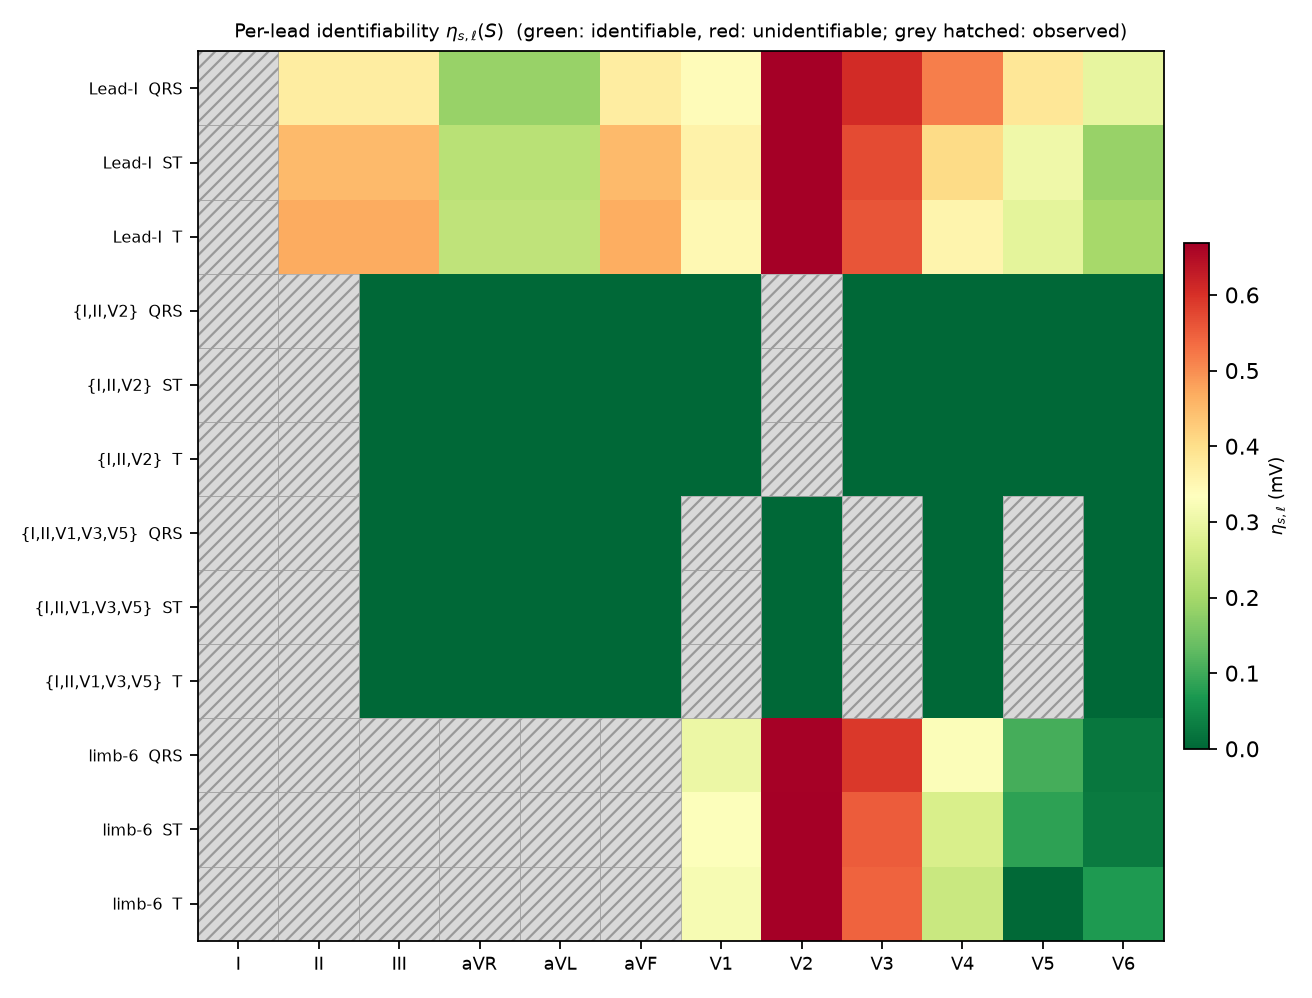
\includegraphics[width=\linewidth]{../results/recoverability_map.png}
  \caption{Recoverability map: normalized identifiability $\tilde\eta_{s,\ell}(S)$ (left,
  dimensionless) and prior-conditional expected ambiguity in mV (right), colorblind-safe
  \texttt{cividis}; grey hatched = observed. For limb-6 all precordial leads are unidentifiable
  ($\eta{>}0$); the fine ST/T ordering is weighting-sensitive (text).}
  \label{fig:map}
\end{figure}

\textbf{Downstream ST cost across reconstructors.} We reconstruct the full 10-second waveform
with three real continuous linear reconstructors (observed leads exact; ST at J$+$60\,ms vs.\ the
isoelectric PR-segment baseline [P offset\,--\,QRS onset], on fiducials from the observed Lead~II
shared between truth and reconstruction; median over beats; the PR-segment baseline fell back to
the pre-QRS window in $\approx\SafetyFallbackPct$\% of beats), and count ST-threshold events ($|$ST$|{\ge}0.1$\,mV; false positive =
crossing in reconstruction not truth, false negative = vice versa; Table~\ref{tab:safety}). On
$\SafetyN$ common records the \emph{total} wrong-event rate has point estimates ranging
$\TotWrongLo$--$\TotWrongHi\%$ across reconstructors and is \emph{dominated by false negatives}
(missed true crossings: limb$\to$precordial recovery smooths ST toward the population), with the
false-positive/false-negative split a reconstructor choice (paired record-bootstrap $\Delta$ on the
FP/FN split, and on the total, in \texttt{results/st\_safety.json}). We do not derive a minimax/Bayes
bound and make no equivalence claim: we report the range of total-error point estimates,
\emph{not} a certified lower bound, and ST-threshold events, not diagnoses. Because the PR-segment
baseline fell back to the pre-QRS window in $\approx\SafetyFallbackPct$\% of beats, the exact ST
magnitudes inherit that delineation limitation.

\begin{table}[t]
\centering\small
\caption{Limb-6 $\to$ precordial (all V1--V6) ST reconstruction, $\SafetyN$ common fold-10
records. FP/FN = false-positive/false-negative ST-threshold crossings (\%); total = FP+FN. FN
dominates (missed crossings); the split is a reconstructor choice. Auto-generated from
\texttt{results/st\_safety.json}.}
\label{tab:safety}
\begin{tabular}{lcccc}
\toprule
reconstructor & FP\,\% & FN\,\% & total\,\% & $|$ST$|$ err (mV) \\
\midrule
dipolar & \FpDipolar & \FnDipolar & \TotDipolar & \ErrDipolar \\
ridge   & \FpRidge   & \FnRidge   & \TotRidge   & \ErrRidge \\
OLS     & \FpOls     & \FnOls     & \TotOls     & \ErrOls \\
\bottomrule
\end{tabular}
\end{table}

\textbf{Truncation-tolerance sensitivity.} Well-posed configurations are $\varrho$-stable
($\{$I,II,V1,V3,V5$\}$ is rank~3 across $\varrho\!\in\!\{10^{-4},\dots,10^{-1}\}$); near-rank
-deficient sets are $\varrho$-sensitive and reported with the $\varrho$-sweep and bootstrap CIs.
A tiny-but-nonzero singular value is exactly identifiable yet $\varrho$-unidentifiable, which is
why we separate exact from $\varrho$-identifiability (Prop.~\ref{thm:perlead}).
\subsection{Baselines and what the map predicts}
Table~\ref{tab:base} reports reconstruction RMSE (mV) of the unobserved target leads under a
\emph{single, identical protocol} for all methods: per-timepoint waveform RMSE on the same
$\NTestFair$ held-out fold-10 records, same segment indices, record-bootstrap CIs. This is
the fair comparison---an earlier draft scored the classical baselines on segment-mean vectors
and the neural baseline on waveforms, which is not comparable. We include a \emph{strong
neural baseline}: an arbitrary-mask conditional 1-D U-Net trained with random lead masks (so
one model serves any configuration, no target-lead leakage), the masked-reconstruction
architecture the reduced-lead literature uses \cite{gradowski2025reveals}.

On a dipole-spanning set the methods form a monotone ladder---prior-mean $\to$ dipolar
(Tier~I) $\to$ per-segment ridge (Tier~I+II) $\to$ U-Net---confirming there is recoverable
non-dipolar content (the calibrated Tier~II layer), yet the strong neural model's margin over
a simple ridge is small (QRS $\FairSpanUnetQRS$ vs.\ $\FairSpanRidgeQRS$\,mV on
$\{$I,II,V1,V3,V5$\}$). The decisive result is on \textbf{limb-6}: \emph{every} reconstructor
degrades sharply, and the U-Net---despite its capacity---reaches only QRS $\FairLimbUnetQRS$,
$\FairUnetLimbSpanRatio\times$ its spanning-set error, still far above what it achieves when
the target is identifiable. No amount of model capacity crosses the identifiability ceiling
the map's $\eta{>}0$ warning marks out \emph{a priori}: limb$\to$precordial morphology is not
recoverable, so a low reconstruction error there would be spurious.

\begin{table}[t]
\centering\small
\caption{Reconstruction RMSE (mV) of target leads, QRS segment, under one identical
per-timepoint protocol ($\NTestFair$ test records). ``dipolar'' = Tier~I; ``ridge'' =
per-segment ridge (Tier~I+II); ``U-Net'' = strong arbitrary-mask neural baseline. Best in
bold. On limb-6 even the neural baseline cannot recover precordial morphology, as $\eta{>}0$
predicts. Numbers auto-generated from \texttt{results/fair\_baselines.json}.}
\label{tab:base}
% AUTO-GENERATED by paper/emit_baseline_table.py -- do not edit by hand.
\begin{tabular}{lcccc}
\toprule
config & prior-mean & dipolar & ridge & U-Net \\
\midrule
$\{$I,II,V2$\}$ & 0.471 & 0.234 & 0.220 & \textbf{0.181} \\
$\{$I,II,V1,V3,V5$\}$ & 0.484 & 0.186 & 0.168 & \textbf{0.164} \\
limb-6 & 0.484 & 0.362 & 0.346 & \textbf{0.239} \\
\bottomrule
\end{tabular}

\end{table}

\textbf{Empirical, not physical, dipole.} On real PTB-XL the estimated $\bm M_s$ shares two
directions with the classical inverse-Dower vectorcardiographic space (principal angles
$2$--$6^\circ$) but its third direction differs materially (max angle $43$--$55^\circ$,
bootstrap CIs excluding small angles). We therefore treat $\bm M_s$ as an \emph{empirical
rank-3 spatial subspace}, not a physical cardiac dipole; the earlier synthetic
``matches inverse-Dower'' check used inverse-Dower to generate the data and is not evidence
on real ECG. All certificate quantities are stated with respect to this estimated subspace.


\section{Legacy supplement: sensitivity and cross-cohort branches}
\label{sec:limits}
\LegacyBanner
Earlier subspace-angle and cross-cohort summaries are exploratory sensitivity analyses.  The new
protocol instead requires external validation of the score--error relationship.
\section{Cross-Dataset Transfer of the Certificate}
\label{sec:cross}
The certificate is a function of the estimated subspace $\bm M_s$ and the selection $S$; a
fair question is whether it is an artifact of one cohort. We re-estimate $\bm M_s$ under the
\emph{same} unified truncated-SVD numerics ($\varrho{=}10^{-2}$) on the independent
Chapman-Shaoxing-Ningbo 12-lead database \cite{zheng2020chapman} (different country, devices,
sampling; $\CrossNchap$ records) and compare to PTB-XL by principal angles and by the
per-configuration recoverability (rank + global $\kappa$ + per-lead $\eta$). We deliberately do
\emph{not} claim ``population independence''; we report what transfers.

\textbf{QRS subspace is transfer-stable.} For QRS the two datasets' rank-3 subspaces are nearly
aligned (max principal angle $\CrossQRSangMax^\circ$). The per-configuration conditioning
transfers for the well-posed sets: $\kappa$ for $\{$I,II,V2$\}$ is $\CrossKapTriplePtb$ (PTB-XL)
vs.\ $\CrossKapTripleChap$ (Chapman) and for $\{$I,II,V1,V3,V5$\}$ $\CrossKapSpanPtb$ vs.\
$\CrossKapSpanChap$; the near-rank-deficient $\{$V1,V2,V3$\}$ transfers less cleanly
($\CrossKapVvvPtb$ vs.\ $\CrossKapVvvChap$), as expected for an ill-conditioned set.

\textbf{limb-6 is effective rank $\CrossLimbRankPtb$ on both cohorts.} Under the unified
truncation the six limb leads span the frontal plane, so $\bm M_{s,S}$ is rank
$\CrossLimbRankPtb$ (the transverse singular value is truncated) on both PTB-XL and Chapman---we
do \emph{not} invert a near-zero singular value into a spurious $10^{5}$-scale $\kappa$.
Precordial unrecoverability is instead flagged, consistently across cohorts, by $\eta{>}0$
(e.g.\ V2 $\eta{=}\CrossLimbEtaVtwoPtb$ on PTB-XL vs.\ $\CrossLimbEtaVtwoChap$ on Chapman). So
the qualitative identifiable/unidentifiable verdict and the well-posed $\kappa$ ordering are
cohort-stable.

\textbf{ST/T third direction does not transfer.} For the low-amplitude segments the third
subspace direction differs sharply between datasets (max principal angle
$\CrossSTang^\circ$ for ST, $\CrossTang^\circ$ for T). We therefore restrict the transfer
claim: the QRS map and the limb-6 verdict are cohort-stable; the ST/T third spatial direction is
cohort-specific and its map should be re-estimated per dataset---the honest scope of transfer,
not a blanket invariance.

\textbf{Sensitivity to duplicated limb leads (\texttt{results/lead\_weighting.json}).} The six
limb leads are exact combinations of I and II, so a 12-lead PCA up-weights frontal-plane content.
Refitting $\bm M_s$ on the 8 algebraically-independent leads and lifting back via the fixed
transform $\bm T$, the \emph{identifiability verdict is robust}: for the spanning sets the
per-lead $\eta$ is unchanged (max $|\Delta\eta|{=}0$; all targets remain exactly identifiable),
and limb-6 precordial leads stay unidentifiable under both fits. The \emph{magnitudes} of the
low-amplitude ST/T subspace are, however, sensitive: the 12-lead and 8-lead ST/T subspaces
differ by large principal angles ($\LWSTang^\circ$/$\LWTang^\circ$) and $\kappa$ can shift
several-fold (e.g.\ ST $\{$I,II,V2$\}$: $\LWKapTwelve\!\to\!\LWKapEight$). We therefore read the QRS map quantitatively and the
ST/T \emph{graded} values qualitatively---the binary identifiable/unidentifiable verdict is
robust; the exact ST/T $\eta$/$\kappa$/ambiguity magnitudes are weighting-dependent.

\section{Legacy supplement: active lead-selection branch}
\label{app:legacy-selection}
\LegacyBanner
The earlier greedy lead-selection analysis optimized a score fitted on one cohort and did not model
electrode placement constraints.  It is not part of the current contribution and makes no selection
or approximation claim.  A future prescriptive study would require a separate Stage~9 protocol,
bootstrap and cross-cohort stability, and physical acquisition constraints.

\section{Legacy supplement: diffusion and null-space branch}
\label{app:legacy-generative}
\LegacyBanner
The following negative-result record concerns a different generative-model question.  It is retained
for transparency and cannot be used to support the primary robust-map claim.
\section{A Negative Result: the Generative ``Fabrication-Objective'' Story Did Not Survive}
\label{sec:generative}
This project began with a stronger claim---that a diffusion reconstructor proves
``fabrication is a property of the objective,'' a certified hallucination. A pre-submission
re-analysis abandoned it. We document the abandonment in full because the negative result is
itself informative and because selective reporting of the earlier (favourable) numbers would
be exactly the failure the certificate is meant to prevent.

\textbf{Setup.} An arbitrary-mask conditional DDPM (12-channel binary mask $+$ observed values;
random-mask training so one model serves any configuration, with explicit leakage tests)
reconstructs $\{$V2,V4,V6$\}$ from $\{$I,II,V1,V3,V5$\}$ under classifier-free-style guidance
weight $w\in\{1,2,4,6\}$ (\texttt{results/gpu\_deficit\_ci.json},
\texttt{realism\_metrics.json}, \texttt{gpu\_oracle\_gate.json}; all lineage-stamped, numbers
auto-generated).

\textbf{(1) The original effect was a configuration-leakage artifact.} The earlier exhibit
reused one model trained on a fixed observed set to score a \emph{different} configuration.
With leakage removed (arbitrary-mask model $+$ leakage guards) and $\NegSeeds$ training seeds,
the generative reconstructor does \emph{not} outperform a simple held-out \emph{ridge
achievability comparator} (a ridge fit on the observed leads, used as an achievability
reference---\emph{not} a Bayes-optimal oracle, since the model can and does exceed it at low
guidance). The deficit $\Delta\rho=\rho_{\text{ridge}}-\rho_{\text{model}}$---how far the model's
target-lead correlation falls below the ridge comparator $\rho_{\text{ridge}}$---is
\emph{monotone} in $w$: mean $\Delta\rho=\NegDrhoone,\NegDrhotwo,\NegDrhofour,\NegDrhosix$ for
$w=1,2,4,6$ (mean over $\NegSeeds$ seeds; SD $\pm\NegStdsix$ at $w{=}6$). It is small and
negative at $w{=}1$ (the model marginally beats the comparator) and grows to a modest but
seed-\emph{significant} $\NegDrhosix$ at $w{=}6$ (95\% $t$-interval $[\NegCIlo,\NegCIhi]$,
\emph{excludes zero}; the model now falls short of the comparator). Guidance thus moves the gap
the \emph{wrong} way for the fabrication story: it does not buy achievability beyond a plain
ridge, it erodes the model's small low-guidance edge and drives it significantly below the
comparator. The previously reported large diffusion advantage does not reproduce.

\textbf{(2) Realism does not improve with guidance---the causal premise is false.} The story
required higher guidance to buy realism at the cost of fidelity. Instead realism is \emph{no
better} at high guidance: from $w{=}1$ to $w{=}6$ the target-lead PSD log-distance rises (V2:
$\RealPSDVtwoLo\!\to\!\RealPSDVtwoHi$; a small dip at $w{=}2$ then a clear rise, so worsening
but not monotone) and the amplitude-Wasserstein distance rises (V2:
$\RealAmpVtwoLo\!\to\!\RealAmpVtwoHi$). The trend is toward \emph{worse} realism on essentially
every target-lead axis (both PSD log-distance and amplitude-Wasserstein rise from $w{=}1$ to
$w{=}6$); there is no monotone realism/fidelity trade to exploit. This is consistent with
fundamental limits on hallucination in inverse problems~\cite{gottschling2026hallucinations} and
the perception--distortion tradeoff~\cite{blau2018perception}: raising perceptual pressure
(guidance) cannot manufacture target-lead information the observed leads do not carry.

\textbf{(3) What is true instead.} The predictable non-dipolar residual is real but modest:
ridge-comparator correlations (\texttt{gpu\_oracle\_gate.json}) are
$\rho\!\approx\!\RidgeRhoVtwoLo$--$\RidgeRhoVtwoHi$ for V2 (QRS/ST) and
$\RidgeRhoLatLo$--$\RidgeRhoLatHi$ for V4/V6---consistent with the calibrated Tier-II
intervals of Sec.~\ref{sec:calib}. So the honest statement is a \emph{graded predictability} of
the residual, calibrated per feature and lead, not a proof of fabrication. We removed the
fabrication-objective claim and rebuilt the paper around the parts that withstand scrutiny.

\textbf{(4) A rigorous, ground-truth-free fabrication audit.} The certificate lets us make the
fabrication idea precise without ground truth. Whatever a reconstruction asserts in the
\emph{unidentifiable} dipole subspace $\bm Q=\bm I-\bm P_{\mathrm{obs}}$ is content the observed
leads cannot fix; we score the fraction of a reconstruction's dipolar energy that lies there,
$\phi=\|\bm M_s\bm Q\hat{\bm d}\|^2/\|\bm M_s\hat{\bm d}\|^2$ (Fig.~\ref{fig:fab}). Principled
reconstructors \emph{abstain}: the dipolar and prior-mean reconstructions have $\phi\!=\!0$
everywhere ($\le\FabAbstainMax$), and even ridge/OLS keep $\phi\!=\!0$ wherever the observation
spans the dipole (limb-6, $\{$I,II,V2$\}$). But on a heavily under-determined single lead the
linear reconstructors fabricate ($\phi\!=\!\FabRidgeLeadIQRS$ for ridge, Lead-I QRS), and the
diffusion model fabricates most of its dipolar content in the provably unrecoverable subspace
($\phi\!\approx\!\FabDiffLeadIlo$) with fabrication \emph{rising with guidance}
($\phi\!:\!\FabDiffLeadIlo\!\to\!\FabDiffLeadIhi$ QRS, $\to\!\FabDiffLeadISThi$ ST as $w{:}1\to6$;
$\phi\!\le\!\FabDiffLimbSix$ on limb-6). This is the defensible, disciplined form of ``fabrication
is a property of the objective'': more guidance manufactures more content the data cannot support,
without improving achievability (point 1)---quantified by the certificate rather than asserted.

\begin{figure}[t]
  \centering
  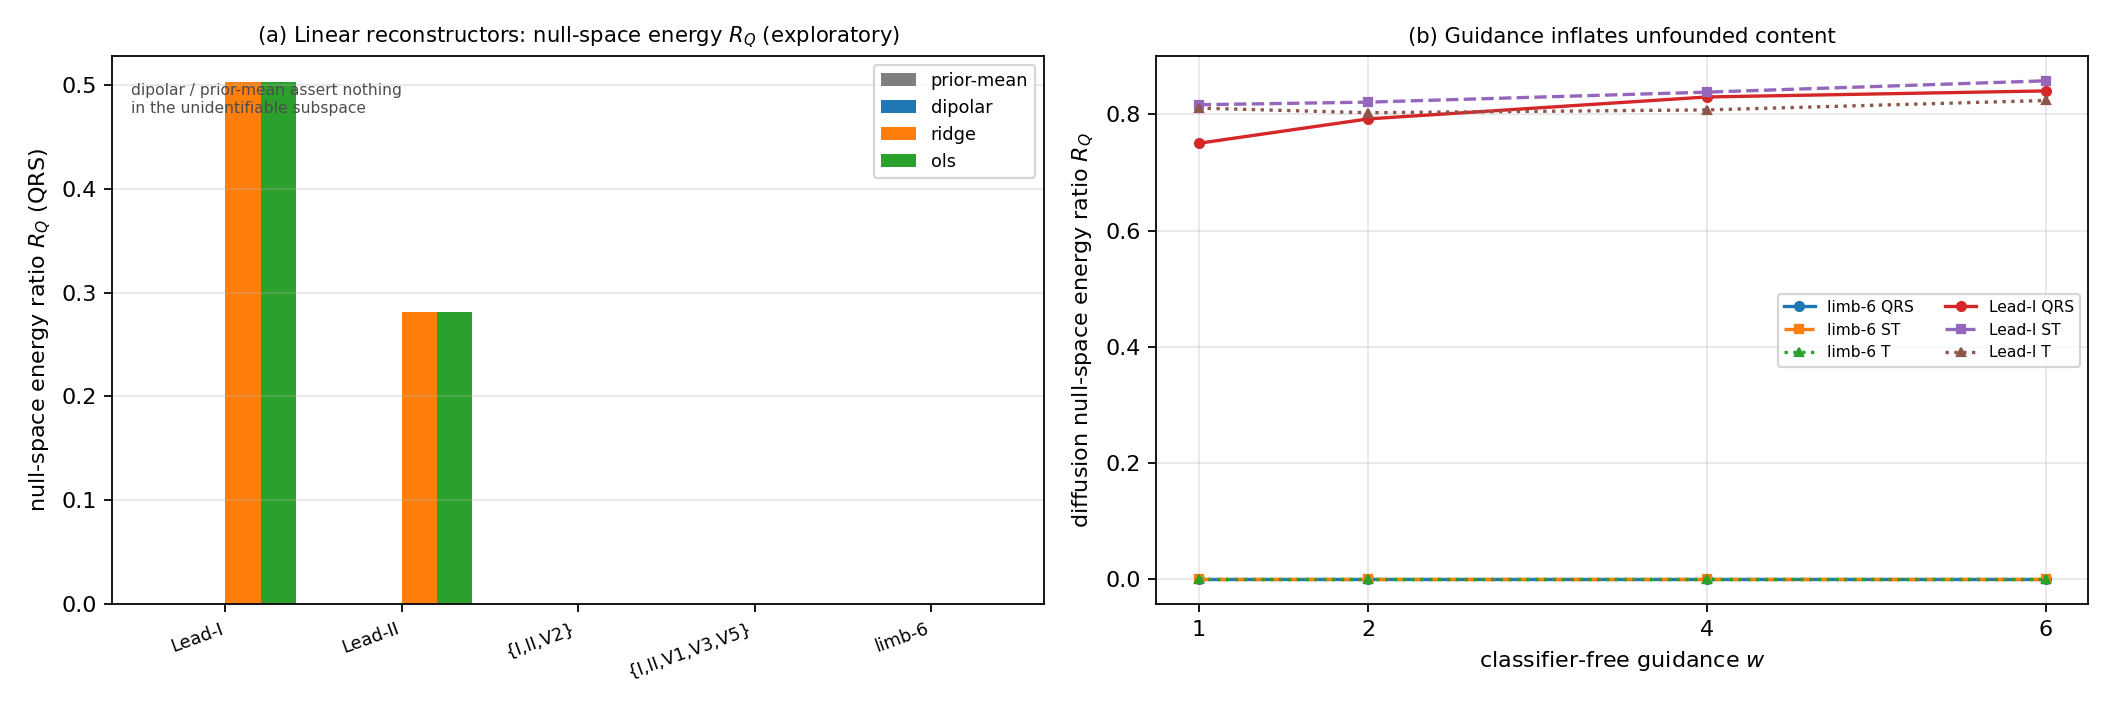
\includegraphics[width=\linewidth]{../results/fabrication_audit_figure.png}
  \caption{\textbf{Null-space dipolar fabrication audit} (ground-truth-free). $\phi$ = fraction of a
  reconstruction's dipolar energy in the certified-unrecoverable subspace $\bm Q$. (a) Linear
  reconstructors: dipolar/prior-mean abstain ($\phi{=}0$); single-lead ridge/OLS fabricate; on
  observation sets that span the dipole (incl.\ limb-6) even ridge/OLS abstain. (b) The diffusion
  model fabricates most of its dipolar content on a single lead and fabrication \emph{grows with
  classifier-free guidance} $w$, while abstaining on limb-6. Regenerated from
  \texttt{results/fabrication\_audit.json}, \texttt{fabrication\_diffusion.json}.}
  \label{fig:fab}
\end{figure}

% ICASSP 2027 permits only references, funding acknowledgments, and this separately titled
% compliance section on page 5. Every sentence below is generated from signed build inputs.
{\footnotesize
\section*{Funding Acknowledgment}
\SubmissionFundingStatement

\section*{Compliance with Ethical Standards}
\SubmissionComplianceStatement

\noindent\textbf{Competing interests.} \SubmissionConflictStatement

\noindent\textbf{AI-assisted tool provenance.} \SubmissionToolDisclosure

\noindent\textbf{Human verification.} \SubmissionHumanVerificationStatement
}


\bibliographystyle{IEEEbib}
\bibliography{refs}
\end{document}
